\chapter{CNIs}\label{chpt:cni}

% Circa 12 pagine

\label{sec:network}

% Since its first appearance, distributed architectures have played a vital role
% in scientific computing. The main idea behind this approach is that if a single
% computing unit is not powerful enough to solve a problem, multiple units can do
% it.
% The reason why this approach is so successful and popular lies in the fact that
% Performing horizontal scaling is always cheaper than vertical scaling.
% However, this approach has a significant drawback: since the computation is
% now distributed, it may be necessary, mainly if the computations performed by
% the different units are not independent, to exchange data between them. This
% introduces a new problem: the network used to perform this inter-node
% communication.

Since its first appearance, distributed architectures have played a vital role
in scientific computing. The main idea behind this approach is that if a single
computing unit is not powerful enough to solve a problem, multiple units can do
it. The reason why this approach is so successful lies in the fact that
Performing horizontal scaling is cheaper than vertical scaling and can go beyond
its limitations. However, a distributed approach has a significant drawback:
data has to be moved between different units through additional dedicated
infrastructure. When everything is distributed, we perform data processing on
different nodes from those where we store it. Furthermore, if the computations
are not independent, it may be necessary to exchange data between nodes
dedicated to the computation. All this additional data motion introduces a new
problem: the network used to perform this inter-node communication.


% This fact may seem trivial, but it is not. Performing this kind of
% operation has a cost, measurable in terms of the significant complexity of the
% infrastructure and, obviously, time. At the beginning of the
% distributed computing era, this was not a big problem since the order of
% magnitude of the time needed to perform this kind of operation was irrelevant
% compared to the time needed to perform the computation.
% However, in the last decade, the situation has started to change. The amount of
% processed data has increased exponentially. However, more importantly, the
% progress in the HPC hardware industry has delivered massive computational power,
% making the time needed to perform the computation itself much smaller.

% In particular, thanks also to the significant adoption of hardware accelerators,
% the time needed to perform the computation has decreased much faster than the
% time needed to perform the inter-node communication, making the latter a real
% bottleneck in modern computation.
% This is a well-known problem, and many vendors have started developing
% faster network technologies, like Infiniband, omni-path, Gigabit Ethernet, and
% so on, to solve this problem. However, this may be not enough.
% This is a well-known problem for anyone who has ever worked with distributed
% systems, since scaling profilation as the one shown in figure \ref{fig:scaling}
% are becoming more and more common.

Moving data has a measurable cost in terms of the significant complexity and
time required for infrastructure. At the beginning of the distributed computing
era, data motion was not a problem since the order of magnitude of time needed
to perform this kind of operation was negligible compared to the time needed to
perform the computation. However, the situation has changed in the last decade,
and we are now in the opposite. Thanks to the significant adoption of hardware
accelerators, the time needed to perform the computation has fallen. We are at a
point where dedicated hardware can process data much faster than the time it
takes to fetch it, making the latter the bottleneck of modern computation. This
bottleneck is well-known, and many vendors have started developing faster
network technologies, like Infiniband, omni-path, Slingshot, and Ultra Ethernet,
to solve this problem. However, more is needed because we are approaching a
situation where anyone working with distributed systems starts to encounter
scaling profilations like the one sketched in figure \ref{fig:scaling}.

\begin{figure}[h]
  \centering
  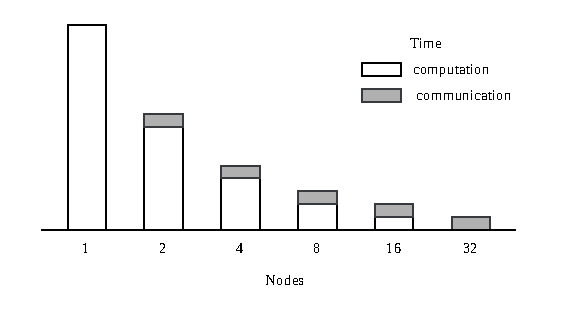
\includegraphics[width=0.85\textwidth]{img/chpt2/scaling}
  \caption{Representation of how the communication time easily becomes the
    bottleneck in modern computation. The figure shows an ideal case where
    the computation time scales linearly with the number of nodes, and the
    communication time remains constant. This is usually not the case since
    dealing with many nodes is usually more complex, and the
    communication time tends to increase with the number of nodes. However, it is
    evident that if the code is parallelizable enough, the computation time
    tends to zero, making the percentage of time spent in communication more and
    more relevant.}
  \label{fig:scaling}
\end{figure}


% Other than the physical limitation imposed by the network technology itself,
% there is another problem that may arise: the software stack used to perform the
% communication. Even the fastest network devices will be slowed up by the
% overhead introduced by the operating system itself and any other software
% responsible for managing those devices.
% Libraries like MPI used to perform communication in HPC, try to optimize this
% step as much as possible, and vendors like Mellanox, Intel, and Cray have started
% to develop their own libraries.

% All this introduction was made to make clear to the reader why all the traction of the
% Container Networking Interface Plugin (CNI Plugin) in this and the following
% chapter is so important and extensive. As will be shown in detail, the CNI is
% a crucial part of the Kubernetes ecosystem, and it is responsible for managing
% the network of the pods.
% Those plugin provides an abstraction layer between the Kubernetes network and
% the underlying network infrastructure, but at the same time, they introduces the
% most significant overhead in the network communication in a Kubernetes cluster.
% Knowing in the details how they work is essential to understand how to optimize
% the network communication in a Kubernetes cluster to not come too early to the
% conclusion as in the past (see section \ref{sec:intro-literature-review}) that
% using a cloud native infrastructure for HPC is not feasible.
% In the very last years some of the most adopted CNIs have been tested in the
% scientific literature, like the ones presented by Kapočius (2020)
% \cite{Kapoius2020}, Kang et al. (2020) \cite{Kang2021}, and finally, the most
% recent and comprehensive survey by Koukis et al. (2024) \cite{Koukis2024}.

Other than the physical limitation imposed by the network technology, another
problem arises with the software stack used to perform the communication. Even
the fastest network devices will be slowed down by the overhead introduced by
the operating system and any other software responsible for managing those
devices.  In the case of HPC, no abstraction needs to be introduced, so
libraries responsible for communication can interface directly with the kernel.
This allows for the development of low-level, highly optimized solutions like
message-passing interface (MPI) implementations. However, this is not feasible
in the cloud paradigm, where a layer of abstraction is always needed. Often,
such a layer takes the name of "Container Networking Interface" Plugin (CNI
Plugin). As will be shown in detail, the CNI is a crucial part of the Kubernetes
ecosystem, and it is responsible for managing the network of the pods. The CNI
plugin provides the network layer to the Kubernetes orchestrator and interfaces
it with the underlying network infrastructure. While this paradigm is needed, if
not to enable networking within the orchestrated containers, it introduces the
most significant overhead in network communications within the cluster.

Through the last decade, the CNI panorama has been very active, and performances
have been one of the main selling points, along with features of all these
software. This interest led to a rich literature in performance analysis
\cite{Kapoius2020,Kang2021, Qi_2021,Koukis2024}. All those studies focused on
performances typical for a web application, such as HTTP connection and SSH
session, seldom expanding their studies in the lower layers typically consumed
by HPC workflows. The main takeaway message is that there is no "\textit{ideal
CNI plugin}" that outperforms all the others in every possible scenario. The
choice of the CNI plugin to use in a Kubernetes cluster may depend on many
factors, such as the hardware used, the specific requirements of the
application, and the time the managing team can dedicate to setup and
maintenance. For this reason, we think that it should be good practice to
perform an assessment of how the Kubernetes cluster behaves to the different
CNIs, like the one presented in the chapter \ref{chpt:osu}, and make the proper
consideration before deploying a production environment. For the specific case
of the ORFEO cluster used for the thesis presented, the CNI plugins considered
and evaluated are Calico, Flannel, and Cilium. The first two were chosen for the
encouraging performance results shown by Koukis \emph{et al.}\cite{Koukis2024},
and the latter for its simplicity and flexibility.

% As it should be reasonable to expect, in all the previous studies there is not a
% "\textit{ideal CNI plugin}" which just outperform all the others in every
% possible scenario. The choice of the CNI plugin to use in a Kubernetes cluster
% may depend on many factors, like the hardware used, the specific requirements of
% the application, and so on. For this reason, according to the authors of this
% thesis, should be considered a good practice to perform an assessment of how the
% Kubernetes cluster react to the different CNIs, like the one presented in the
% chapter \ref{chpt:osu} \textit{"CNIs comparison and assessment"} and make the
% proper consideration to do a wise choice.
% For the specific case of the ORFEO cluster used for the thesis presented, the
% considered CNIs plugin evaluated are Calico, Flannel, and Cilium. The first two
% for the very promising results in \cite{Koukis2024} (in particular Cilium claims
% to be an high performance CNI) and the latter one for its adoption due to its
% simplicity and flexibility.


\section{Node-to-node communication in Kubernetes}\label{sec:node2node}

From the Red Hat system administration guide:
\textit{``A CNI plugin is responsible for inserting a network interface into the
    container network namespace (e.g., one end of a virtual ethernet (veth)
    pair) and making any necessary changes on the host (e.g., attaching the
    other end of the veth into a bridge). It then assigns an IP address to the
    interface and sets up the routes consistent with the IP Address Management
    section by invoking the appropriate IP Address Management (IPAM) plugin.''
} \cite{redhat-cni}.


\begin{figure}[H]
  \centering
  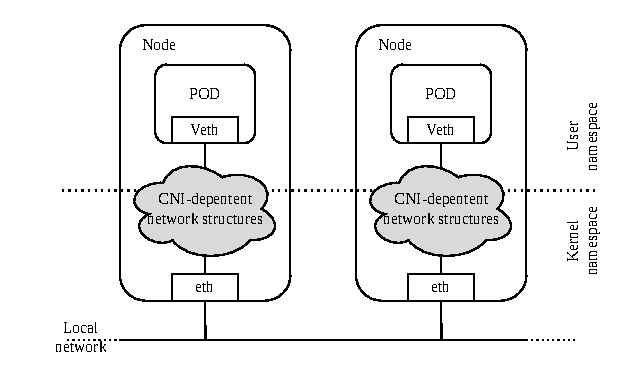
\includegraphics[width=0.9\textwidth]{img/chpt2/CNI-generic}
  \caption{Graphical schematization of the definition provided in
    \cite{redhat-cni} about how a CNI plugin works. In every pod (in figure one
    per node only for simplicity and clarity) a VETH is inserted, and the CNI
    acts as a man in the middle between the pod and the host to make possible to
    the containers in the pod to use the underlying network infrastructure to
    reach the other nodes.}
  \label{fig:cni-generic}
\end{figure}


This is a very high-level definition, since ``making any necessary changes on
the host'' is a very broad statement. This is due to the fact that all the
modification performed are very CNI plugin-specific. Different solutions usually
adopts different approach to solve the same problem, making impossible to
formulate a more detailed definition without referring to a specific CNI plugin.
In the rest of this chapter, the details about how the considered CNI plugins
(Calico, Flannel and Cilium) work under the hood will be presented.


\subsection{Calico}\label{subsec:calico}

Calico is a widely used CNI solution created by Tigera and built on the Border
Gateway Protocol(BGP) \footnote{BGP is a standard communication protocol for
Autonomous Systems (AS). It facilitates the exchange of routing and reachability
information, determining the best path for communication traffic
\cite{BGPnistdef}.}. The installation process for Calico is straightforward and
can be executed using either the helm package manager or Tigera's dedicated
operator. After the installation, the Kubernetes cluster will spawn the
following pods: \texttt{calico-apiserver} in a namespace of the same name and
\texttt{calico-kube-controllers} and \texttt{calico-node} pods in the
\texttt{calico-system} namespace. The \texttt{calico-apiserver} allows sysadmins
to manage calico resources directly using \texttt{kubectl}. In contrast, the
\texttt{calico-kube-controllers} pod monitors the Kubernetes API and performs
actions based on the cluster state.

The principal pod is the \texttt{calico-node}, deployed using a DaemonSet on
each node, which runs three internal daemons \cite{calicodoc}:

\begin{enumerate}
  \itemsep0em
  \item \textit{Felix}: Manages routes, access-control lists (ACLs), and all
    other requirements for providing connectivity for the endpoints on the host
    node. It is responsible for:
    \begin{itemize}
      \itemsep0em
      \item \textit{Interface management}: Programs information about interfaces
        into the kernel to ensure the correct handling of traffic from the
        endpoint. This includes ensuring the host responds to ARP (Address
        Resolution Protocol) requests from each workload with the host's MAC and
        enabling IP forwarding for managed interfaces.
        It also monitors interfaces to ensure that programming is applied at the
        appropriate time.
      \item \textit{Route programming}: Programs routes to the endpoints on its
        host into the Linux kernel FIB (Forwarding Information Base), ensuring
        incoming packets destined for those endpoints are correctly forwarded.
      \item \textit{ACL programming}: Programs ACLs into the Linux kernel to
        control traffic between endpoints and prevent circumvention of Calico's
        security measures.
      \item \textit{State reporting}: Provides network health data, reporting
        errors and problems when configuring its host. This is then written to
        the datastore for visibility to other components and network operators.
    \end{itemize}
  \item \textit{BIRD}: Retrieves routes from Felix and distributes them to BGP
    peers on the network for inter-host routing. It runs on each node that hosts
    a Felix agent and acts as an open-source internet routing daemon. The BGP
    client is responsible for:
    \begin{itemize}
      \itemsep0em
      \item \textit{Route distribution}: Distributes routes inserted into the
        Linux kernel FIB by Felix to other nodes in the deployment, ensuring
        efficient traffic routing.
      \item \textit{BGP route reflector configuration}: Configures BGP route
        reflectors for large deployments to act as a central point for
        connecting BGP clients, ensuring efficient route advertisement without
        passing endpoint data through them.
    \end{itemize}
  \item \textit{confd}: Monitors the Calico datastore for changes to BGP
    configuration and global defaults such as AS numbers, logging levels, and
    IPAM information. It is an open-source, lightweight configuration
    management tool that dynamically generates BIRD configuration files based on
    datastore updates, triggering BIRD to load the new files.
\end{enumerate}



% The Calico declined version of figure \ref{fig:cni-generic} is represented in
% figure \ref{fig:cni-calico}.
% Here is reported the step-by-step path of a network packet that has to be sent
% from pod A in node A to pod B in node B in this configuration:

When using Calico, the user can configure the previously described components to
achieve different network architectures. This study will limit ourselves to a
typical generic setup for on-prem and on-the-cloud installation: an IPIP overlay
mode combined with BGP for inter-node routing. We confined the cluster to a
single L2 network to avoid paring BGP to our network infrastructure. In this
case, the Calico declined version of figure \ref{fig:cni-generic} is represented
in figure \ref{fig:cni-calico}. 

Here we report the step-by-step path of a network packet that has to be sent
from pod A in node A to pod B in node B in this configuration:

\begin{enumerate}
  \item \textit{Pod A Sends a packet}: Pod A needs to communicate with pod B,
    which is in another node. It generates a network packet destined for pod B,
    which exists only now in pod A's network namespace. The communication, from
    the point of view of pod A, is done using a virtual Ethernet interface
    (\texttt{veth0}).
  \item \textit{The net packet enters in node A root network namespace}: This is
    possible thanks to Calico CNI-plugin, which takes care of attaching to every
    veth0 interface of every pod a virtual Ethernet interface in the host
    network namespace (\texttt{cali}).
  \item \textit{Felix configures the host's routing table}: On node A, Felix has
    preconfigured routes in the host's routing table based on the IP addresses.
    Using these routes makes it possible to forward the packet to the correct
    next hop, in this case, in another node in the cluster: node B.
  \item \textit{Checks the network policies}: Before proceeding, Felix also
    ensures that all the needed security policies are enforced (e.g., Kubernetes
    NetworkPolicies). The allowed packet proceeds to the next step if the checks
    are successful.
  \item \textit{BIRD Advertises Routes via BGP}: The BGP client running on node
    A advertises the IP address ranges (CIDRs) of the pods on node A to all the
    other nodes in the cluster using BGP. Similarly, node A learns about the pod
    in node B through the BGP announcements from the BIRD instance running on
    that node.
  \item \textit{Packet is routed to node B}: the route learned by the BGP
    client in the previous step are installed in the host routing table by BIRD,
    letting node A know how to reach the pod on the other nodes.
  \item \textit{Packet is ready to be sent to node B}: The packet from pod A is
    forwarded based on the routing table entries that were set up by Felix and
    learned via BIRD. Since node A knows how to reach node B (thanks to the BGP
    routes learned by BIRD), the packet is forwarded to the network interface
    \texttt{eth0} that leads to node B.
    %% TODO an educated guess suggests me that at this step the packet is
    %% encapsulated via IPIP
  \item \textit{confd checks}: the daemon queries the Kubernetes API and etcd
    from the control plane, ensuring that if there are any changes (e.g., new
    pods, some changes in the topology) node A is not aware of. If so, the BIRD
    configuration will be updated accordingly. Even if confd does not directly
    handle the packet, it plays a crucial role in maintaining the accuracy of
    the routing, ensuring that routing informations are always up-to-date.
  \item \textit{Packet reaches node B}: The packet goes through the (local)
    network and reaches node B. On that node, the Linux routing table
    (configured by Felix) determines that the packet should be delivered to pod
    B.
  \item \textit{Packet delivered to pod B}: The packet enters pod B via its
    virtual Ethernet interface and reaches the application running inside the
    pod.
\end{enumerate}

\begin{figure}
  \centering
  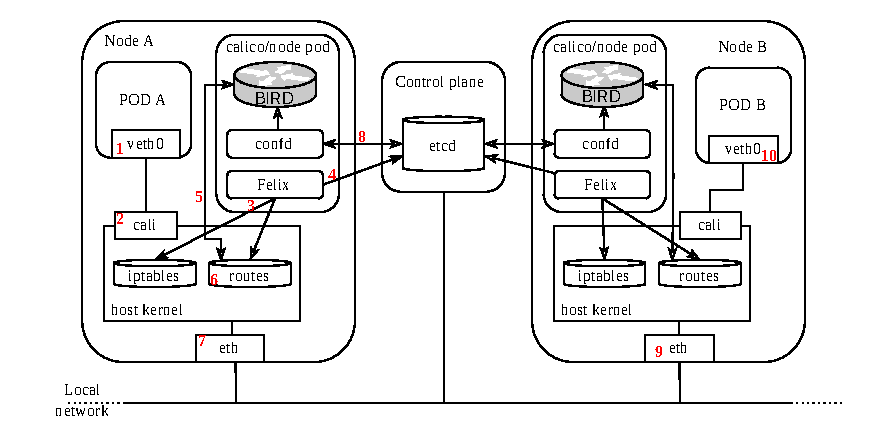
\includegraphics[width=\textwidth]{img/chpt2/CNI-calico}
  \caption{Graphical schematization of how the Calico CNI plugin acts in a
    Kubernetes cluster. In red there are reported the steps with the same
    numeration of the list above to make clear the path of a network packet.}
  \label{fig:cni-calico}
\end{figure}

\subsection{Flannel}\label{subsec:flannel}

Flannel is the second CNI plugin that was taken as a candidate for the
Kubernetes infrastructure deployed in the ORFEO cluster. Flannel is a simple and
widespread solution developed at CoreOS under the Red Hat umbrella science 2018.
Thanks to its simplicity, minimalism, and portability, it has become the default
CNI plugin in many Kubernetes distributions, among which K3s\footnote{K3s is an
open-source project developed by Rancher under the Suse. This project is often
mentioned as a more straightforward and lighter version of K8S} and the Amazon
Elastic Kubernetes Service (EKS).

Unlike Calico, which relies on BGP routing, Flannel's approach is based on a
``static'' partitioning of the pod CIDR combined with iptables for packet
routing (leveraging features such as destination natting). Host routing across
the nodes is obtained, by default, by using the Virtual Extensible LAN (VXLAN)
protocol \cite{flannel-github}\footnote{  VXLAN is a network virtualization
technology that provides a way to encapsulate Layer 2 packets within Layer 4
packets. This technology introduces an abstraction layer of indirection that
allows overcoming the limitations of the VLAN technology, like the maximum
number of VLANs that can be created in a network or, more importantly, in this
context, introduces the possibility of having multiple instances that share the
same physical network but are logically separated \cite{VXLANnistdef}.}

% The installation of Flannel is also straightforward, and it can be performed
% either by applying the manifest file provided by the official repository or by
% using the official helm chart. In this case the installation process deploys
% very few components with respect to Calico. Flannel will spawn (using a DaemonSet)
% just one pod called \texttt{kube-flannel} per node in a dedicated namespace with
% the same name. These pods are responsible for managing the network configuration
% of the node, ensuring seamless communication between pods across the cluster.


% The main component of Flannel is \texttt{flanneld}, a binary agent that runs on
% each node in the cluster. This daemon has among his duties:

The installation of Flannel is straightforward, and it can be performed by
applying the manifest file provided by the official repository or by using the
official helm chart. As fewer features are implemented in this case, very few
components are needed. Flannel will spawn (using a DaemonSet) just one pod
called \texttt{kube-flannel} per node in a dedicated namespace with the same
name. These pods are responsible for managing the network configuration of the
node, ensuring seamless communication between pods and across the cluster. The
main component of Flannel is \texttt{flanneld}, a binary agent that runs on each
node in the cluster. This daemon, is responsible, among others, for the following
operations:

\begin{itemize}
  \item \textit{Subnet Management}: Each node in the Kubernetes cluster is
    assigned a unique subnet by \texttt{flanneld}, ensuring no IP address
    conflicts between pods across different nodes. This subnet is used to
    allocate IP addresses to pods on the node.
  \item \textit{Encapsulation and Routing}: Depending on the backend
    configuration (e.g., VXLAN), \texttt{flanneld}
    encapsulates the packets destined for other nodes within an overlay network.
    In the case of VXLAN, for instance, packets are encapsulated with a VXLAN
    header and sent across the network to the appropriate destination node.
 \item \textit{IP Address Management (IPAM)}: Flannel uses a simple,
   etcd-backend IP address management system to allocate and track IP addresses
   assigned to pods. This ensures each pod has a unique IP address within the
   cluster and facilitates seamless communication between pods.
  \item \textit{Network Configuration Updates}: \texttt{flanneld} continuously
    monitors the etcd datastore for any changes in network configuration (e.g.,
    new nodes being added to the cluster, changes in subnet allocations) and
    dynamically updates the routing tables and network configurations on the
    nodes.
\end{itemize}

The general scheme proposed in figure \ref{fig:cni-generic} is contextualized
for the Flannel CNI plugin in figure \ref{fig:cni-flannel}.  Analogously to the
previous section, let us have a look at the journey a packet has to do to be
sent from pod A in node A to pod B in node B in a Kubernetes installation
equipped with Flannel:

\begin{enumerate}
  \item \textit{Pod A generates a packet}: Pod A, running in node A, generates a
    packet destined for pod B, which is being executed in node B. In this phase,
    the packed still exists only in the network namespace of pod A, from whom
    point of view, will be sent using his virtual Ethernet interface
    (\texttt{veth0}).
  \item \textit{Packet forwarding to node A's bridge}: The packet leaves pod A
    through its veth interface, which is one end of a virtual Ethernet pair. The
    other end of this veth pair is attached to node A's network bridge
    (\texttt{cni-bridge}) set up by Flannel.
    In this phase, the bridge on node A forwards the packet based on the IP
    address.
    % The flannel pod is typically connected to this bridge too (\texttt{flannel.1}).
    % This is not true, you can check it with brctl show.
    % At a first glance the iptable is responsible for changing the routing
  \item \textit{Encapsulation}: On node A, Flannel operates as an overlay
    network and encapsulates the packet using VXLAN to create a virtual L3 network
    over the physical one. The original packet is encapsulated inside a new packet
    with the following additional information:
    \begin{itemize}
      \item Source IP: The IP address of node A.
      \item Destination IP: The IP address of node B.
      \item Payload: The original package which must be sent from pod A to pod B.
    \end{itemize}
  \item \textit{Packet transmission over the physical network}: the host kernel
    handles the encapsulated package, performing a node-to-node communication
    and sending it to node B using the physical network infrastructure.
  \item \textit{Decapsulation on node B}: Once the packet arrives at node B, the
    Flannel instance running on that node decapsulates it. The decapsulation
    process extracts the original packet, with pod A's IP as the source and pod
    B's IP as the destination.
  \item \textit{Forwarding the packet to pod B}: After the decapsulation, the
    bridge on node B forwarded the packet to the appropriate virtual ethernet
    interface corresponding to pod B.
  \item \textit{Packet reception in pod B}: Finally, pod B receives through its
    veth interface the packet as if it was sent directly from pod A without any
    knowledge of the encapsulation/decapsulation process and the underlying
    network hops.
\end{enumerate}

% A relevant aspect it must be mentioned is that unlike the other considered the
% Flannel CNI plugin does not provide complete and exhaustive documentation. The
% most similar thing to documentation is a collection of markdown files in a
% \texttt{Documentation} folder in the official GitHub repository, which is more
% focused on explaining all the possible ways to configure the CNI plugin rather
% than how it works under the hood. However, since its popularity, many other
% resources are available online, like dedicated blogs and articles.

A relevant aspect that we must mention is that, unlike the other CNIs considered
within this work, the Flannel CNI plugin does not provide extensive
documentation. The available information is more focused on covering all the
possible ways to configure the CNI plugin rather than how it works under the
hood. Nevertheless, since its popularity, many other resources are available
online, like dedicated blogs and articles.


\begin{figure}
  \centering
  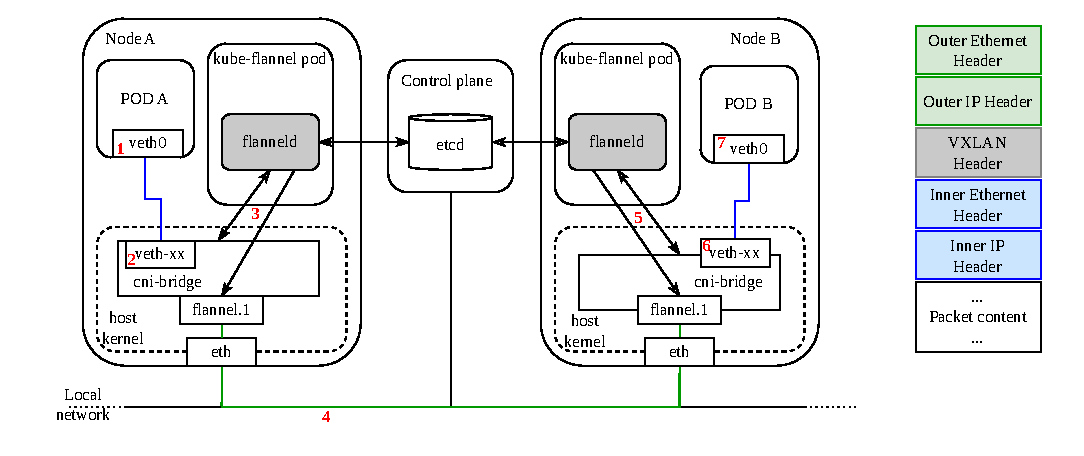
\includegraphics[width=\textwidth]{img/chpt2/CNI-flannel}
  \caption{Graphical schematization of how the Flannel CNI plugin acts in a
    Kubernetes cluster. In red there are reported the steps with the same
    numeration of the list above to make clear the path of a network packet.
    On the right, a reconstruction of the network package transmitted from node
    A to node B in step 4. The color of the various components added and removed
    during the encapsulation/decapsulation process are reported also in the main
    diagram in the involved components.
  }
  \label{fig:cni-flannel}
\end{figure}

\subsection{Cilium}\label{subsec:cilium}

% The last candidate of this study is the Cilium CNI plugin. Cilium is a powerful and advanced
% open-source CNI plugin that has among its supporters companies of the caliber of
% Google, Datadog, and Red Hat, to mention a few.
% Despite being a relatively new project, it has gained much traction in the
% Kubernetes community, to the point that it has become the default choice in
% Google Kubernetes Engine (GKE) for the network policy enforcement.

% What makes Cilium so attractive is probably its statement declaration of being a
% CNI plugin focused on high network performance and security.
% This is achieved by Cilium's unique approach to networking, which, unlike other
% traditional CNI solutions, leverages eBPF\footnote{
%   eBPF (extended Berkeley Packet Filter) is a technology that allows the
%   in-kernel execution of user-defined programs without modifying the kernel
%   source code, loading dedicated kernel modules, and without the need to reboot
%   the machine to apply the changes. Initially developed by Berkeley University
%   for packet filtering tasks, it has evolved and is now adopted in a wide range
%   of situations \cite{Hedam2021}. The main advantage of eBPF is that it allows
%   the execution of programs in kernel space, which is expected to be much
%   faster. In very short, the process is similar to a Just-In-Time (JIT)
%   compilation, where the eBPF program is compiled into a set of instructions
%   that are executed by a sort of virtual machine in the kernel
%   space\cite{Sharaf2022}.
% } technology to provide a deeper level of control and visibility over the
% network traffic.

The last candidate for this study is the cilium CNI plugin. Cilium is another
powerful and feature-rich open-source CNI plugin that has companies of the
caliber of Google, DataDog, and Red Hat among its developers. Despite being a
relatively new project, it has gained much traction in the Kubernetes community.
Recently, it has also become the default choice in the Google Kubernetes engine
(GKE), a valid reason to consider it a production-ready solution when deploying
new clusters. 

What we believe makes Cilium so attractive is its statement declaration that it
is a CNI plugin focused on high network performance and security. This goal is
achieved by Cilium's unique approach to networking, which, unlike other
traditional CNI solutions, leverages extended Berkeley Packet Filter
(eBPF\footnote{eBPF is a technology that allows the in-kernel execution of
user-defined programs without modifying the kernel source code, loading
dedicated kernel modules, and without the need to reboot the machine to apply
the changes. Initially developed by Berkeley University for packet filtering
tasks, it has evolved and is now adopted in a wide range of situations
\cite{Hedam2021}}). The main advantage of eBPF is that it allows the execution
of programs in kernel space, which can run faster and have higher privileges
than those in the user space. In very short, the process is similar to a
Just-In-Time (JIT) compilation, where the eBPF program is compiled into a set of
instructions that are executed in a send-boxed environment in the kernel
space\cite{Sharaf2022}. This technology allows for higher control and visibility
over the network traffic, strongly impacting latency.

% The installation process of Cilium can be performed using the helm package
% manager for Kubernetes; however, it is strongly recommended to use the dedicated
% \texttt{cilium install} command provided by a dedicated CLI tool.
% In fact, the Cilium project provides a dedicated CLI tool written in Go which
% can be used to install, manage, and monitor the Cilium CNI plugin in a
% Kubernetes more comfortably\footnote{To be fair, Calico project has a similar
%   tool called \texttt{calicoctl} but it usage avoidable at all since also its
%   documentation does not report it anywhere but in its dedicated page}.
% The installation ends up with the spawning of the \texttt{cilium-operator} pod
% plus one \texttt{cilium} and one \texttt{cilium-envoy} pods per node in the
% cluster; unlike the other CNIs, all these pods are not spawned in a dedicated
% namespace but the \texttt{kube-system} one is used. The following list
% summarizes the purpose of each of them \cite{ciliumdoc-components,
%   ciliumdoc-envoy}:

The installation process of Cilium can be performed using the helm package
manager for Kubernetes; however, the documentation strongly recommends using the
dedicated \texttt{cilium install} command provided by a dedicated CLI tool. The
Cilium project provides a dedicated CLI tool written in Go which can be used to
install, manage, and monitor the Cilium CNI plugin in Kubernetes more easily
\footnote{We didn't mention it earlier, but Calico has a similar tool called
\texttt{calicoctl}. However, such a tool is not in pair with what Cilium can
offer, and since its usage can be avoided, we decided to do so}. The
installation ends up with the spawning of the \texttt{cilium-operator} pod plus
one \texttt{cilium} and one \texttt{cilium-envoy} pods per node in the cluster;
unlike the other CNIs, all these pods are not spawned in a dedicated namespace
but the \texttt{kube-system} one is used. The following list summarizes the
purpose of each of them \cite{ciliumdoc-components, ciliumdoc-envoy}:

% \begin{itemize}
%   \itemsep0em
%   \item \textit{Operator pod}: As every operator in rubbernecks is responsible orchestrating all those aspects that should logically be handled once and for all, the entire cluster rather than case-specific decisions that should be taken node per node. Technically, it is not essential in any network policy decision. A cluster could, in theory, continue to function even when that pod is temporary unavailable. However, the operator's absence could lead to the following: is tempraly unaviability shouldent impact operations
%     \begin{itemize}
%       \itemsep0em
%       \item delays in the IP Address Management (IPAM), which could lead to postponed scheduling of new workloads when the operators need to assign additional IP addresses.
%       \item failure of updating the key-value datastore (etcd) with values, which may lead to agents declaring unhealthiness state and restarting.
%     \end{itemize}
%   \item \textit{Cilium agent pods}: They are the core of the Cilium CNI plugin. A DaemonSet guarantees their presence among every node. They accept the Kubernetes configuration through the API and enforce the desired networking, service load-balancing, and security policies. Moreover, they wait for events from the orchestrator to learn about the current cluster situation (new pods, new nodes, ...) and react accordingly, managing the eBPF programs used in the host kernel to control all network access in/out of those containers.
%   \item \textit{Envoy pods}: They are used as host proxy for enforcing network policies specified in the Kubernetes NetworkPolicies cluster specifications. They are responsible for proxying all L7 traffic to and from the pods in the node, keeping a separate process concerning the agent one. The main advantages of this separation are:
%     \begin{itemize}
%       \itemsep0em
%       \item possibility of restarting the agent (e.g., for upgrades) without impacts for the live traffic since it will be proxied via envoy
%       \item separate CPU and memory limits for performance isolation
%       \item Dedicated health probes and logs for the two components
%     \end{itemize}
% \end{itemize}
\begin{itemize}
  \item \textit{Operator pod}: Like every operator in Kubernetes, it directs all
    aspects concerning Cillium. From pod scheduling to resource monitoring and
    policy updating across the cluster. Technically, it is not essential in any
    network policy decision. A cluster could, in theory, continue to function even
    when that pod is temporarily unavailable. However, the operator's absence for a
    prolonged amount of time could lead to infrastructure instability.
  \item \textit{Cilium agent pods}: They are the core of the Cilium CNI plugin.
    A DaemonSet guarantees their presence among every node. They accept the
    Kubernetes configuration through the API and enforce the desired networking,
    service load-balancing, and security policies. Moreover, they wait for events
    from the orchestrator to learn about the current cluster situation (new pods,
    new nodes, ...) and react accordingly, managing the eBPF programs used in the
    host kernel to control all network access in/out of those containers.
  \item \textit{Envoy pods}: They are used as host proxy for enforcing network
    policies at the application layer, as specified in the Kubernetes
    NetworkPolicies cluster specifications. They are responsible for proxying all L7
    traffic to and from the pods in the node, keeping a separate process concerning
    the agent one.  The main advantages of this separation are:
    % TODO Double check on this.
    \begin{itemize}
      \item possibility of restarting the agent (e.g., for upgrades) without impacts for the live traffic since it will be proxied via envoy
      \item separate CPU and memory limits for performance isolation
      \item Dedicated health probes and logs for the two components
    \end{itemize}
\end{itemize}

% It is notable to know that by default, several features are not enabled, for
% example: the possibility of performing inter-cluster communication with
% \texttt{cilium-clustermesh} or the capability of Cilium to perform network
% packet encapsulation similar to what happens in the case of Flannel. The latter
% becomes essential when deploying on cluster where there is no control on the
% host network.

It is notable to know that by default, several features are not enabled for
example: the possibility of performing inter-cluster communication with
\texttt{cilium-clustermesh} or the capability of Cilium to perform network
packet encapsulation similar to what happens in the case of Flannel. The latter
becomes essential when deploying on an infrastructure where there is no control
over the hosts network.

% The Cilium declined version of figure \ref{fig:cni-generic} is reported in
% figure \ref{fig:cni-cilium}. To be consistent with the structure adopted in
% section \ref{subsec:calico} and \ref{subsec:flannel}, there is reported also
% for the Cilium case, the step-by-step path a network packet has to go through to
% be sent from pod A in node A up to pod B in node B:

The Cilium declined version of figure \ref{fig:cni-generic} is reported in
figure \ref{fig:cni-cilium} as previously done with Calico \ref{subsec:calico}
and Flannel \ref{subsec:flannel}. We also report the step-by-step path a network
packet has to go through to be sent from pod A in node A up to pod B in node B:


\begin{enumerate}
  \itemsep0em
  \item \textit{pod A needs to communicate with pod B}: Pod A in node A needs to
    communicate with pod B in node B. It generates a packet destined for pod B,
    which starts its existence in pod A's network namespace.
  \item \textit{Packet leaves pod A}: The packet exits pod A through its virtual
    Ethernet interface (\texttt{veth}). On the other tip of the veth pair, a
    virtual Ethernet interface in the host network namespace is created by
    Cilium to intercept the outgoing packet using eBPF hooks
    (\texttt{veth-cilium}).
  \item \textit{Policy check}: The agent on node A ensures that the packet is
    allowed to proceed checking the Kubernetes NetworkPolicies. If it is
    authorized,  the process continues; otherwise, the packet is dropped.
  \item \textit{Routing decision}: The Cilium Agent, using its eBPF maps,
    determines the destination for the packet, in this case on another node
    (obviously, it could be in the same node).
  \item \textit{Packet transmission}: The packet is sent over the physical
    network to node B. By default, Cilium assumes that the underlying network
    supports direct routing. If not, the encapsulation (e.g., VXLAN) must be
    enabled for overlay networking.
  \item \textit{Packet arrival at Node B}: The packet arrives at Node B's
    network interface. The Cilium Agent on Node B intercepts the incoming packet
    using eBPF hooks.
  \item \textit{Second policy check}: The Cilium agent on node B performs a
    second control to be sure that the packet is allowed to enter pod B.
    If that is not the case, it will drop.
  \item \textit{Packet delivery}: The agent uses eBPF to deliver the packet
    directly to pod B's network namespace, sending it to the pod through its
    virtual Ethernet interface.
\end{enumerate}

\begin{figure}
  \centering
  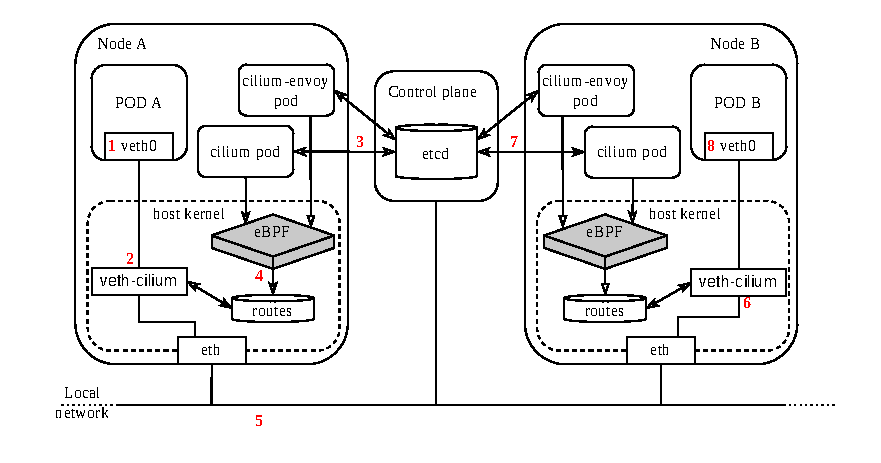
\includegraphics[width=\textwidth]{img/chpt2/CNI-cilium}
  \caption{Graphical schematization of how the Cilium CNI plugin acts in a
    Kubernetes cluster. In red there are reported the steps with the same
    numeration of the list above to make clear the path of a network packet.}
  \label{fig:cni-cilium}
\end{figure}


% As it was possible to appreciate the set of possibilities to configure the host
% operating system and network to guarantee the communication nodes in a
% Kubernetes cluster is incredibly vast.
% It should be reasonable to expect that such marked difference in the
% implementation behind the hood will inevitably reflect in different performance
% of communication.
% In the following chapter it will be shown a possible way to assess the
% performance of the CNIs in a Kubernetes cluster, to express a quantitative
% evaluation.

This chapter explored various possibilities for configuring the host operating
system and network to guarantee that the communication nodes are in Kubernetes.
We choose three of the most widespread and supported CNIs in the field, but many
more solutions are available to suit different needs and niches. We covered
Calico, a comprehensive and well-established solution, with the disadvantage of
not being straightforward to configure in all its parts. We then went through
Flannel, a minimalistic but easy-to-use solution, and Cillium, the most
cutting-edge that takes innovative approaches by leveraging eBPF whenever
possible to increase performance. Based on the discussion above, it is
reasonable to expect that such marked differences in the implementation behind
the hood of network management will inevitably reflect in different
communication performances. In the following chapters, we will assess the
performance of the CNIs in a Kubernetes cluster from an HPC perspective using
well-recognized benchmarks and a data science perspective to see how
infrastructural choices impact commonly used frameworks.
